\chapter[Referencial Teórico]{Referencial Teórico}

Para inicializar o nosso Referencial teórico de forma concisa em que se alinhe com o que foi proposto com o capítulo 1, é imprescindível abordar o contexto e papel da Fertilização In Vitro, qualidade dos embriões e desafios associados, além de evidenciar como a Inteligência Artificial pode auxiliar a aprimorar as taxas de sucesso de gravidez e minimizar os fatores de risco relacionados a abortos, problemas cromossômicos, além de reduzir os impactos emocionais e físicos associados a esses desafios.

\section{Fertilização In Vitro}

Registros históricos mostram que as civilizações antigas, como a grega que realizavam rituais e peregrinações para deidades e a egípcia que adotavam talismãs e amuletos para invocar bençãos dos deuses da fertilidade, deram uma grande importância à fertilidade, entendendo como uma bênção divina e continuação da linhagem da sociedade. Cada civilização possui métodos que buscavam a fertilidade, apesar de serem considerados como crenças em contraste com a ciência, ainda refletem que essa busca sempre foi um interesse enraizado nas culturas humanas \cite{moura2020}

Com o passar dos anos e da evolução do campo científico, essa busca pela fertilidade teve um avanço significativo na biologia e medicina. “A primeira inseminação artificial de que se tem registro foi realizada pelos árabes em 1332, em equino”, porém os primeiros resultados em seres humanos, com inseminação de sêmen no útero, foram obtidos apenas no final do século XVIII \cite{moura2020}. Dos anos 1970 em diante, essa técnica vem sendo bastante utilizada e toda essa trajetória de desenvolvimento corroborou para a revolução dos limites da concepção assistida, contribuindo cada vez mais as taxas de sucesso dessas reproduções assistidas.

A Reprodução Assistida (RA), depois de décadas sendo aprimorada, é definida como um Conjunto de métodos aplicados por médicos especializados com o objetivo de auxiliar ou possibilitar a reprodução em homens e mulheres com esterilidade ou infertilidade. \cite{souzamarise2024}. Ao citar o tema de reprodução assistida, é comum que venha à mente a Fertilização In Vitro (FIV).

A FIV é a técnica mais conhecida e mais complexa da RA. Ela promove a união, em ambiente laboratorial, do óvulo —célula reprodutiva feminina, também conhecida como gameta feminino— ao espermatozóide —célula reprodutiva masculina, ou gameta masculino— \cite{associacaobrasileira2024}. Em termos mais técnicos, é a coleta de um óvulo (ou ovócito) maduro, fertiliza-o em laboratório e transfere o embrião —fase inicial do desenvolvimento de um organismo após a fertilização, quando o óvulo e o espermatozóide se combinam— resultante para o útero.  O ano de 1978 foi marcado por uma grande evolução na medicina reprodutiva: o nascimento do primeiro bebê concebido pela FIV. Louise Brown, “o neném de proveta”, nasceu no Reino Unido, com a técnica de fertilizar um óvulo fora do corpo humano, realizada pelos médicos Patrick Steptoe e Robert Edwards \cite{corleta2010}. 

Após esse feito histórico, a medicina reprodutiva foi transformada e abriu novas oportunidades para pessoas que enfrentam essa dificuldade de fertilidade. Esses fatos citados destacam como, ao longo do tempo, a humanidade sempre procurou superar a infertilidade. Hoje, com a combinação dos avanços da medicina e da tecnologia, nos concede não apenas efetuar a fertilização in vitro, mas também realizar exames detalhados para descobrir a qualidade genética dos embriões, auxiliando ainda mais as taxas de sucesso da FIV. 

No próximo tópico, discutiremos a análise de embriões, procedimento esse que auxilia a identificar possíveis anomalias e aumentar as chances de concepção saudável, e a sua importância na seleção para a FIV.

\section{Métodos de Avaliação Genética em Reprodução Assistida}

Para evoluir na constatação de doenças genéticas na plore relacionadas ao número de cromossomos (Aneuploidia), são os métodos de avaliação genética em RA que fazem a análise para identificar possíveis anomalias, já que “a qualidade dos embriões é o fator mais crítico para o sucesso da fertilização in vitro” \cite{wang2019}, pois desempenham um papel expressivo para evitar os abortos, visto que estudos indicam que até 50\% de perdas gestacionais são devidas a anormalidades cromossômicas \cite{scienceofbiogenetics2024}. Após anos de pesquisa, o progresso na testagem genética vem permitindo cada vez mais diagnósticos precisos e técnicas mais avançadas, complexas e atreladas a tecnologia, como a Testagem Genética Pré-implantacional, conhecido como PGT.

Pelo final do século XX, o método do PGT começou a ser usado para realizar o rastreamento de doenças genéticas que possuíam uma alta taxa de incidência nas populações de amostra \cite{yang2024}. Com ele, foi propiciada a triagem de embriões antes da implementação, permitindo a seleção de embriões que possuíam menos riscos \cite{scienceofbiogenetics2024}. Atualmente, existem três tipos de PGT: “(1) para aneuploidia (PGT-A), como Síndrome de Down e Síndrome de Turner; (2) para defeitos monogênicos/gene único (PGT-M), como distrofia miotônica e fibrose cística; (3) e para rearranjos estruturais cromossômicos (PGT-SR)” \cite{yang2024}. Neste estudo, a atenção está voltada para a Testagem Genética Pré-implantacional para Aneuploidias (PGT-A), que distingue alterações no número de cromossomos dos embriões para melhorar a seleção embrionária com o objetivo de evitar a aneuploidia.  

O médico especilaista, por meio deuma entrevista, explica que o PGT-A é um procedimento embrionário realizado em embriões durante as etapas de FIV que analisa o número de cromossomos em cada embrião antes de transferi-los, aumentando as porcentagens de uma transferência de FIV sucedida, garantindo que os embriões tenham o número correto de cromossomos \cite{ramalho2024}. Também ressaltou que um embrião considerado “normal” (euploide), os mais desejados pois produzem a maior chance de uma gravidez bem-sucedida, possui 23 pares de cromossomos oriundos do esperma e 23 pares oriundos do óvulo, com um total de 46 cromossomos. O embrião considerado “anormal” (aneuploide) tem uma contagem a mais em algum cromossomo, assim, tendo 3 cópias, em oposição às duas que deveria ter \cite{cnyfertility2024}. Mas afinal, como o PGT-A performa? Explicaremos em 5 etapas para melhor entendimento:

\begin{itemize}
    \item \textbf{Etapa 1: Biópsia de tecido}
    \begin{itemize}
        \item Nessa primeira etapa de teste, é realizada depois dos estágios de estimulação ovariana—processo em que medicamentos hormonais são usados para estimular os ovários—, coleta de óvulos, fertilização e desenvolvimento embrionário em FIV. A partir do momento em que os embriões chegam em um estágio de desenvolvimento de aproximadamente 5 a 7 dias após a fertilização, é realizado uma biópsia—retirada de algumas células de um embrião—de tecido, com a consequência da retirada de uma amostra das células de cada embrião congelado para realizar testes genéticos \cite{cnyfertility2024}. 
    \end{itemize}

    \item \textbf{Etapa 2: Envio de amostras e congelamento de embriões}
    \begin{itemize}
        \item Após a etapa 1, essas amostras de tecido retiradas das células de cada embrião são enviadas para o laboratório de genética, é lá que se realizam os testes de verificação. Os embriões são congelados e armazenados até a hora da transferência do embrião selecionado \cite{cnyfertility2024}. 
    \end{itemize}

    \item \textbf{Etapa 3: Análise cromossômica PGT-A}
    \begin{itemize}
        \item Depois que as amostras de tecido chegarem no laboratório e da análise dos cromossomos, o PGT-A é concluído. Na análise, os embriões passam por exames relacionados a anormalidades cromossômicas \cite{cnyfertility2024}. 
    \end{itemize}

    \item \textbf{Etapa 4: O Relatório Genético}
    \begin{itemize}
        \item Ao concluir a análise, o laboratório envia um relatório genético que tem os detalhes dos status de cada embrião selecionado para teste, contendo nesse documento o número de cromossomos de cada. O médico especialista em fertilidade conferirá os resultados e relatará os resultados obtidos com o paciente em questão \cite{cnyfertility2024}. 
    \end{itemize}

    \item \textbf{Etapa 5: Seleção de embriões e transferência congelada}
    \begin{itemize}
        \item Baseando-se nos resultados detalhados no relatório genético, o especialista em fertilidade escolherá o(s) embrião(ões) saudável(eis) para a transferência. O(s) embrião(ões) selecionado(s) será(ão) então descongelado(s) e preparado(s) quando for a hora da transferência do embrião \cite{cnyfertility2024}. 
    \end{itemize}
\end{itemize}

O resultado que o PGT-A entrega para pacientes que o utilizam é a classificação dos embriões, a qual possui 3 tipos de resultados diferentes para cada embrião. Eles são classificados com um dos três resultados potenciais do teste: Euplóide (normal)—todas as células amostradas do embrião têm 46 cromossomos—, mosaico (parcialmente normal, parcialmente anormal) —algumas células que foram testadas no embrião são normais, algumas são anormais—e aneuplóide (anormal) —todas as células obtidas da biópsia tinham um número anormal de cromossomos—\cite{cnyfertility2024}. A Figura~\ref{fig:ResultadosPGT} ilustra os resultados do PGT-A e suas respectivas probabilidades de sucesso gestacional.

\begin{center}
    \begin{figure}[h]
        \captionsetup{font=footnotesize, justification=centering, labelsep=period, position=above}
        \caption{Resultados do PGT-A e suas respectivas probabilidades de sucesso gestacional}
        \label{fig:ResultadosPGT}
        \centering
        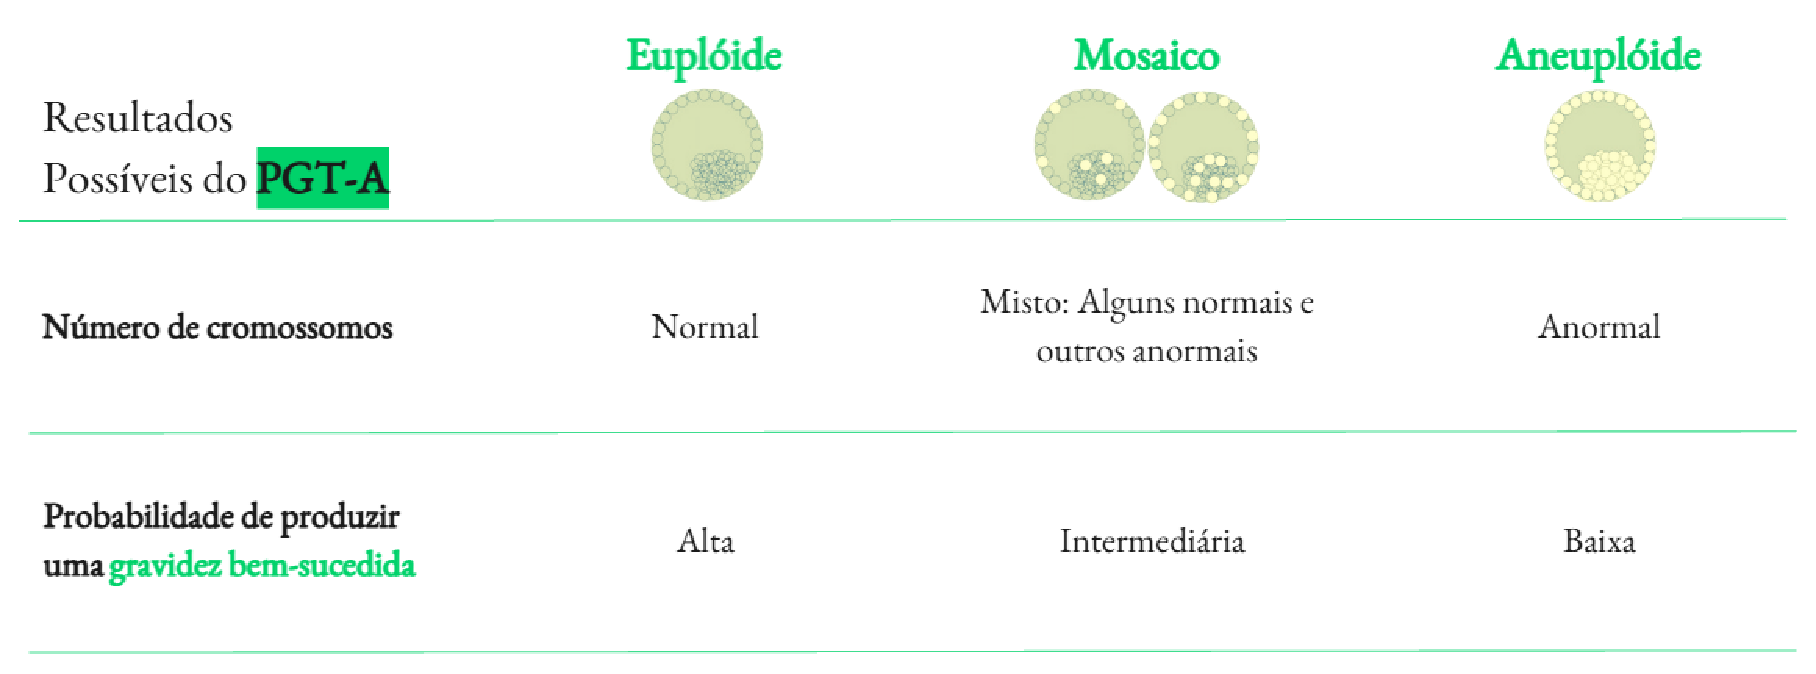
\includegraphics[scale=0.5]{figuras/ResultadosPGT.pdf}
        \vspace{0.3cm} 
        \scriptsize{Fonte: Autoras (2024)}
    \end{figure}
\end{center}

Dessa forma, é investigado qual é o melhor embrião entre os selecionados para a análise genética, tudo partindo de uma biópsia, como descrito na etapa 1. O PGT é um procedimento relativamente complexo pois exige uma biópsia dos embriões, onde qualquer dano mínimo deve ser evitado e por esse motivo é considerado um método invasivo e apresenta riscos potenciais ao embrião \cite{yang2024}.

Um método invasivo na FIV são aqueles que utilizam técnicas de operação direta no embrião ou em células que vão formar o embrião. Um exemplo é a biópsia citada nas etapas do PGT-A, em que se realiza uma remoção da célula do embrião para analisar geneticamente, \citeonline{phillips2024} levantam aflições de que a remoção dessas células em crescimento possa impedir o desenvolvimento do embrião em questão, comprometendo os resultados neonatais, pois as técnicas de micromanipulação para biópsia não são totalmente isentas de riscos, como citado por \citeonline{leaver2019}. “Além disso, a natureza invasiva da biópsia requer uma manipulação de embriões demorada por embriologistas experientes, tornando este um procedimento caro para os pacientes” \cite{phillips2024, leaver2019}. Ainda que o PGT-A permita detectar aneuploidias e expandir as porcentagem de gravidez bem-sucedida, se tem a chance de afetar o potencial de implantação do embrião. Por esses motivos apresentados, métodos não-invasivos estão sendo estudados para disponibilizar alternativas eficientes e seguras, se tornando cada vez mais significativas. Um exemplo de técnica não-invasiva é o Time-Lapse System {-} Sistema de Time-Lapse (TLS).

O TLS é uma técnica que Exige capturar imagens contínuas dos embriões em desenvolvimento em intervalos regulares, sem alterar o ambiente de cultivo. \cite{moustakli2024}. De acordo com o médico especilaista, o especialista em fertilidade podem utilizar essa técnica para monitorar o momento das divisões celulares e regularidade disso, observando momentos importantes do crescimento e, com esse monitoramento contínuo, conseguindo distinguir um embrião euplóide ou aneuplóide de acordo com seu padrão desenvolvimento. De acordo com \citeonline{moustakli2024}, o TLS dispõe-se oferecer insights valiosos sobre a saúde e o potencial de desenvolvimento dos embriões, utilizando técnicas não invasivas como a biópsia de embriões. alguns estudos mostram que o TLS e as pontuações morfocinéticas podem aumentar as taxas de implantação e gravidez clínica em relação aos métodos tradicionais. \cite{boucret2021}.

Os dados morfocinéticos de embriões coletados pelo TLS oferecem uma oportunidade para melhorar a escolha de embriões em tratamentos de FIV. Supondo uma IA que tem a capacidade de analisar esses dados, teríamos a possibilidade de identificar padrões e predizer a porcentagem, de euploidia. Isso representaria uma abordagem não-invasiva e mais acessível financeiramente. Ao pensar nessa IA e esse ser o objetivo do trabalho presente, é imprescindível compreender como a IA poderia ser aplicada nesse contexto e como ela poderia ser capaz de fazer essa abordagem. 

\section{Inteligência Artificial}

As dificuldades em definir IA não são, portanto, o resultado de alguma deficiência ou descuido, mas surgem do fato de que fomos incapazes de determinar precisamente qual inteligência desejaríamos replicar artificialmente \cite{sheikh2023}. Dessa forma, definimos a Inteligência Artificial como sistemas que exibem comportamento inteligente ao analisar seu ambiente e tomar ações {–} com algum grau de autonomia {–} para atingir objetivos específicos \cite{sheikh2023}. 

Na medicina reprodutiva, a IA tem se mostrado promissora na melhoria de processos como a fertilização in vitro (FIV). Essa busca por imitar a inteligência humana e entender seus processos cognitivos levou ao desenvolvimento de diversas abordagens, entre elas o Aprendizado de Máquina (Machine Learning, ML), que envolve a capacidade de computadores de interpretar grandes volumes de dados, construir modelos baseados nesses dados e, assim, gerar hipóteses ou previsões sobre o mundo ao seu redor \cite{russell2016}. Na medicina, algoritmos podem ser treinados para reconhecer padrões genéticos em embriões, classificar o melhor embrião para implantação e prever características genéticas de novos embriões. 

Os métodos de ML são geralmente classificados em três tipos principais: aprendizado supervisionado, aprendizado não supervisionado e aprendizado por reforço. Neste estudo, opta-se pelo aprendizado supervisionado como abordagem principal, dada sua eficácia na análise de dados rotulados, permitindo decisões mais precisas e embasadas para otimizar os tratamentos de FIV.

O aprendizado supervisionado consiste no treinamento de algoritmos com base em conjuntos de dados rotulados, nos quais as variáveis de entrada (inputs) e os resultados esperados (outputs) já são conhecidos. O algoritmo aprende a correlacioná-los de forma eficiente \cite{russell2016}, ajustando seus parâmetros com base nas diferenças entre previsões e resultados reais \cite{trask2019}. Uma técnica amplamente usada dentro do aprendizado supervisionado é a classificação, cujo objetivo é atribuir rótulos ou classes pré-definidas aos dados. Por exemplo, no contexto da medicina reprodutiva, um modelo pode ser treinado para diferenciar embriões euploides e aneuploides, aprendendo a reconhecer padrões associados a cada grupo \cite{izbicki2020}.

De maneira geral, um algoritmo de aprendizado supervisionado separa o banco de dados em três subconjuntos: treinamento, validação e teste \cite{izbicki2020}. Na fase de treinamento, o algoritmo identifica padrões nos dados de entrada e os associa às classes desejadas \cite{izbicki2020}. Na validação, um subconjunto de dados não utilizado no treinamento avalia o desempenho do modelo \cite{izbicki2020}, permitindo ajustes nos hiperparâmetros. Após resultados satisfatórios, o conjunto de testes mensura métricas como acurácia, recall e precisão, garantindo o desempenho esperado \cite{izbicki2020}.

A seleção aleatória das amostras para treinamento, validação e teste é uma boa prática \cite{izbicki2020}, evitando problemas decorrentes de ordenações previamente estabelecidas nos bancos de dados. Isso assegura uma visão representativa e imparcial dos dados, fundamental para a construção de modelos robustos e confiáveis \cite{izbicki2020}.

Para a exploração inicial dos dados, utilizaremos o modelo k-Nearest Neighbors (kNN) como ponto de partida, conforme apresentado no livro Aprendizado de Máquina: Uma Abordagem Estatística \citeonline{izbicki2020}. Caso o desempenho e a confiabilidade do kNN não sejam satisfatórios, passaremos a avaliar outros modelos de classificação, como Regressão Linear e Naive Bayes, seguindo esse processo iterativo até encontrarmos um modelo que atenda aos critérios desejados. Se alguns desses modelos demonstrarem resultados satisfatórios, não será necessário explorar os demais.

\section{O Algoritmo K-Nearest Neighbor (KNN)}
O algoritmo K-Nearest Neighbor (KNN) é, em essência, um dos algoritmos mais simples e populares em aprendizado supervisionado, sendo utilizado principalmente em tarefas de classificação e regressão \cite{zhang2016}. Sua principal característica é classificar uma nova observação com base nas classes de seus k vizinhos mais próximos previamente rotulados \cite{zhang2016}. O KNN pode ser considerado um modelo não paramétrico, pois não faz suposições a respeito da distribuição dos dados, o que o torna bastante versátil para uma diversidade de problemas \cite{zhang2016}. É também um algoritmo de aprendizado "preguiçoso" já que não ocorre um processo explícito de aprendizado \cite{zhang2016}.  Então, o algoritmo armazena os dados de treinamento e, na hora de fazer uma predição usa a distância da nova observação para cada exemplo discretamente do conjunto de treinamento para descobrir qual classe ou valor alvo deve usar \cite{zhang2016}.

O desempenho do KNN dé dependente da escolha de k, que são o número de vizinhos que são considerados na classificação \cite{zhang2016}. Valores muito pequenos de k podem a levar a overfitting, já que o modelo se torna sensível ao ruídos contidos nos dados. Valores muito grandes, por sua vez, podem resultar em underfitting pela perda de padrões locais importantes \cite{elkan2011}. Nesse trabalho, utilizaremos num primeiro momento k = 3 e k = 5 para avaliar o desempenho do modelo. Estes valores são adequados uma vez que eles capturam padrão locais sem exagerada sensibilidade ao ruído. Caso necessário, faremos o ajuste no parâmetro k com base nos resultados do conjunto de validação, pois o conjunto de validação é empregado especificamente para otimizar hiperparâmetros.

A métrica de distância adotada foi a distância Euclidiana, uma das mais simples e mais utilizadas. Essa é uma escolha adequada para pequenos conjuntos de dados e de baixa dimensionalidade, como o utilizado neste estudo. Para tais condições a distância euclidiana capta similaridades com eficiência, além de facilitar a interpretação dos resultados \cite{elkan2011}.

O funcionamento do KNN pode ser resumido em três etapas principais de acordo com o \citeonline{elkan2011}:
\begin{itemize}
    \item Armazenar os exemplos de treinamento com suas respectivas etiquetas.
    \item Calcular a distância entre uma nova observação e todos os exemplos armazenados, utilizando uma métrica de similaridade, como a distância Euclidiana.
    \item Selecionar os k vizinhos mais próximos e determinar a classe mais frequente entre eles, atribuindo-a à nova observação.
\end{itemize}

Essa abordagem de classificação por maioria contribui para mitigar o impacto de ruídos ou valores extremos \cite{elkan2011}. Uma prática comum para definir o valor de k é utilizar a raiz quadrada do número total de observações no conjunto de treinamento, embora ajustes específicos sejam feitos dependendo do problema e do conjunto de dados \cite{elkan2011}.

\section{Regressão Linear}
A regressão linear é uma técnica estatística utilizada em aprendizado de máquina para expressar relações entre variáveis e para realizar previsões baseadas em dados passados \cite{rodrigues}. É uma abordagem essencial em aprendizado supervisionado, oque visa detectar padrões e criar modelos generalizáveis para dados até então inexistentes \cite{soto}. Segundo \citeonline{santos2007},  é usada para quantificar a associação entre as variáveis, usando frequentemente o coeficiente de correlação de Pearson para avaliar a força e a direção dessa relação. A regressão linear pode ser dividida em dois tipos principais: regressão linear simples e regressão linear múltipla \cite{soto}.

Em um contexto de IA, a regressão linear simples estabelece uma relação matemática entre uma variável dependente \( Y \) e uma única variável independente \( X \), descrita pela equação:
\[
Y = \beta_0 + \beta_1 X + \epsilon,
\]
onde \( \beta_0 \) representa o intercepto, \( \beta_1 \) é o coeficiente angular que expressa a taxa de variação de \( Y \) em relação a \( X \), e \( \epsilon \) é o termo de erro aleatório \cite{rodrigues}. Modelos mais complexos, como a regressão linear múltipla,permitem a inclusão de mais de uma variável independente, aumentando assim a capacidade preditiva e explicativa do modelo \cite{rodrigues}.

A regressão linear é um método paramétrico que requer a suposição de uma relação linear entre as variáveis, o que pode torna-la restritiva quando os padrões não são lineares. Entretanto, técnicas de pré-processamento, como transformações de variáveis e inclusão de termos polinomiais, podem contornar essa limitação e aumentar a capacidade de generalizar do modelo \cite{montgomery2009}.

\section{Naive Bayes}
O Naive Bayes é um algoritmo de classificação que se baseia no Teorema de Bayes para estimar a classe mais provável de uma instância, utilizando a probabilidade condicional dos atributos observados \cite{rish2001}. Ele é chamado de "naive" (ou ingênuo) porque parte da suposição de que os atributos são condicionalmente independentes dado a classe. Em outras palavras, presume que a presença ou ausência de um atributo não afeta os outros atributos. Embora essa suposição não seja totalmente realista em muitas situações do mundo real, o algoritmo ainda apresenta resultados impressionantes em diversas aplicações práticas \cite{rish2001}.

De acordo com \citeonline{zhang2004}, o Naive Bayes determina a probabilidade de uma instância pertencer a uma classe específica analisando a distribuição condicional dos atributos. Mesmo com a simplificação imposta pela suposição de independência, o algoritmo muitas vezes alcança resultados comparáveis a métodos mais avançados. O Naive Bayes é particularmente eficaz em problemas de classificação de texto, como análise de sentimentos e classificação de documentos, e em tarefas de diagnóstico médico, como detecção de doenças com base em sintomas ou resultados de exames \cite{rish2001}.


Segundo \citeonline{zhang2004}, A ideia central do Naive Bayes é calcular a probabilidade de uma instância $X = \{x_1, x_2, \dots, x_n\}$ pertencer a uma classe $C_k$ utilizando a fórmula:

$$P(C_k|X) = \frac{P(X|C_k) \cdot P(C_k)}{P(X)}$$

Como o denominador $P(X)$ é constante para todas as classes, o foco do cálculo está em maximizar o numerador, que é proporcional a $P(C_k) \cdot \prod_{i=1}^{n} P(x_i | C_k)$, onde $P(x_i | C_k)$ representa a probabilidade condicional de cada atributo $x_i$, dado a classe $C_k$. O algoritmo calcula essas probabilidades para cada classe e atribui a instância à classe com a maior probabilidade \cite{zhang2004}. 

Em resumo, o Naive Bayes é uma solução simples, rápida e incrivelmente eficaz para muitos problemas de classificação, mesmo quando a suposição de independência não é completamente verdadeira. Essa combinação de praticidade e desempenho o torna uma escolha popular em áreas como processamento de linguagem natural e diagnóstico médico.

\section{Identificação de Padrões Morfocinéticos e Predição de Euploidia com IA e Trabalhos Correlatos}

Os dados que são coletados pela tecnologia do TLS, são chamados de “dados morfocinéticos”, que são definidos como “dados do desenvolvimento dos embriões” \cite{oliveira2024}. Essa informação reunida proporciona noções detalhadas sobre o padrão do desenvolvimento e divisão celular embrionário. Atualmente, após recorrentes estudos sobre esses dados, sabe-se que as “características morfocinéticas dos embriões têm sido associadas à avaliação de sua potência de desenvolvimento”, ou seja, se um embrião analisado pelo TLS tenha um melhor desenvolvimento, ele terá mais probabilidade de ser euplóide, pois um bom desempenho de um embrião é capaz de prever a implantação \cite{yuan2023}.

Os modelos de TLS, de acordo com \citeonline{yuan2023}, tem uma avaliação contínua na etapa do desenvolvimento embrionário por meio de suas imagens e, por observações estáticas, monitora as características do embrião, como tempo e padrões de divisão celular, fornecendo uma base para prever a euploidia. O TLS por si só, não opera com a IA, mas é frequentemente mesclado com essa tecnologia para maiores análises. Um exemplo é o estudo do \citeonline{yuan2023}, o artigo “Development of an artifcial intelligence based model for predicting the euploidy of blastocysts in PGT‐A treatments” o qual teve como objetivo utilizar o TLS e desenvolver um modelo de IA usando uma técnica de regressão logística, para predizer a euploidia de blastocistos—fase do desenvolvimento embrionário que ocorre após a clivagem do óvulo fertilizado—em tratamentos de PGT-A, ajudando a identificar embriões com maiores possibilidades de serem geneticamente normais antes da etapa de transferência. O modelo foi avaliado com uma boa precisão, indicando que ele consegue distinguir entre embriões euploides e aneuploides.

Outro estudo é o de \citeonline{souzarebeca2022}, “Análise da ploidia de embriões humanos por meio da inteligência artificial com o uso de variáveis de morfologia, morfocinética e variáveis relacionadas com a paciente”, também descreve o uso de IA para fazer a predição da ploidia de embriões, classificando os embriões como euplóides e aneuplóides. Para realizar isso, o estudo também combinou dados morfológicas, morfocinéticas e parâmetros clínicos, como o \citeonline{yuan2023}. O modelo utilizado por \citeonline{souzarebeca2022}foi uma rede neural artificial (RNA), treinada justamente para classificar os embriões como citado.

Divergente do trabalho de Zhenya Yuan \cite{yuan2023} e de Rebeca Colauto Milanezi de Souza \cite{souzarebeca2022}, que possuem o objetivo de fazer uma previsão binária de euploidia (mostrando se o embrião em estudo é euploide ou não), o modelo que propomos realizar neste trabalho em questão visa prever a porcentagem de aneuploidia. Com essa diferença de resultado, permitimos uma avaliação mais específica da saúde genética do embrião analisado, ofertando um indicador quantitativo em vez de uma classificação binária.

Para fazer a predição da porcentagem de euploidia, planejamos [citar o modelo de IA que iremos fazer], visando otimizar a precisão da predição, enquanto o modelo dos artigos citados usam uma técnica de regressão logística voltada em previsões binárias.

Com essas diferenças citadas, temos o objetivo de criar uma alternativa menos invasiva e mais acessível para a seleção de embriões na FIV.
